\begin{figure}[H]
	\centering
	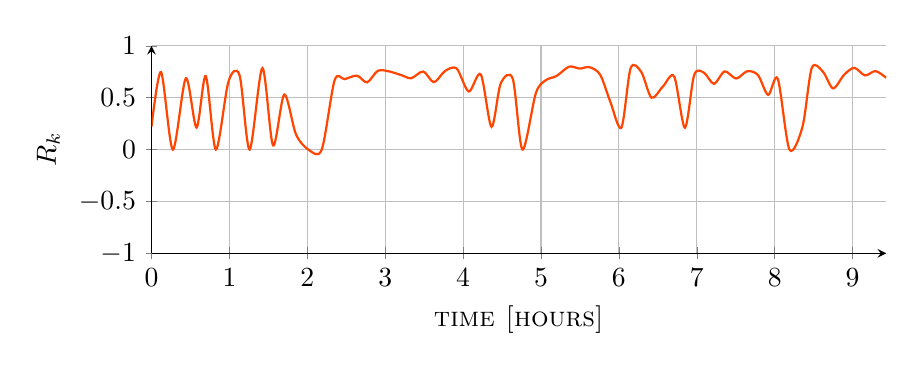
\begin{tikzpicture}
		\begin{axis}[xlabel=\textsc{time [hours]}, ylabel=\textsc{$R_k$}, axis lines=left, grid=major, width=0.9\linewidth, height=12em, ymax=1, ymin=-1]
			\addplot +[mark=none, OrangeRed, thick, smooth] table {
				0.0 0.2210062658266289
				0.12212250000000001 0.7468668542199443
				0.2737058333333333 0.0
				0.44047722222222224 0.6869620634023401
				0.5779966666666667 0.21286318759604017
				0.6963466666666667 0.7077868444361323
				0.8264455555555557 0.0
				0.9877913888888888 0.6553212452037385
				1.1302583333333334 0.7158510962920959
				1.2596577777777778 0.0
				1.4233241666666665 0.78555627833894
				1.560173611111111 0.04031338324190967
				1.7040897222222222 0.5305620645899788
				1.8537841666666666 0.1488366952153271
				2.0139519444444445 0.0
				2.184928888888889 0.0
				2.349692777777778 0.6664427520935514
				2.4791897222222223 0.6790041274095348
				2.637886111111111 0.7123404281741427
				2.7675711111111108 0.6478700713029528
				2.9053605555555557 0.7594913370969733
				3.0537152777777776 0.752626025078389
				3.2100541666666667 0.7165654240441105
				3.3342336111111113 0.6876651438457947
				3.488079722222222 0.7525415707447769
				3.625195833333333 0.6495492115272051
				3.768566111111111 0.7577619062129486
				3.917341388888889 0.7813094792254222
				4.072168055555555 0.5600353040444446
				4.227070277777778 0.7238485747394433
				4.3643025 0.21938184789788054
				4.483167222222222 0.637269512447288
				4.6377825 0.6810954402079779
				4.761978333333333 0.0
				4.9326711111111115 0.5410141600336178
				5.0568905555555554 0.6665433418313889
				5.200257222222222 0.7094159473919907
				5.359889722222222 0.7991117628450763
				5.497729166666667 0.7805775194061032
				5.622027777777777 0.7941215038593585
				5.7592469444444445 0.7218907820667307
				5.888871666666666 0.46286973832844835
				6.0322125 0.21199964894663628
				6.150851111111111 0.7850060226676104
				6.28825138888889 0.746433721275909
				6.418372777777778 0.5000044377566547
				6.566317222222222 0.6093952408434717
				6.7101894444444445 0.7032758499029006
				6.847278888888889 0.21065111766446987
				6.966089444444444 0.7184723832610289
				7.090011944444445 0.7420709094784211
				7.220004444444444 0.6339869249371339
				7.357285555555555 0.7533785641918216
				7.505467222222222 0.6847902950843516
				7.649001944444445 0.7556133453827891
				7.785635277777778 0.717565494444211
				7.9156458333333335 0.5273703354112835
				8.040086666666667 0.6809371503428069
				8.189387777777778 0.0
				8.356989166666667 0.2213466618076342
				8.475808333333333 0.7865802633570821
				8.619317777777779 0.7502291438019768
				8.749226944444445 0.590075638462533
				8.892430833333334 0.7224383394486307
				9.022673055555556 0.7875511127001008
				9.159330277777778 0.7148638548736087
				9.2954025 0.7564852933138435
				9.43203138888889 0.6912593534609529
			};
		\end{axis}
	\end{tikzpicture}
	\caption{Hyper-parameters optimization plot for the category classifier based on neural network.}
	\label{fig:optimization_category_neural_network}
\end{figure}
\begin{table}[H]
	\centering
	\begin{tabular}{ll}
		\toprule
		\textsc{hyper-parameter} & \textsc{value}\\
		\midrule
		\verb|lr| & 0.0027014308955057255\\
		\verb|module__layers| & 4\\
		\verb|module__neurons_per_layer| & 434\\
		\verb|module__p| & 0.1292524544974843\\
		\bottomrule
	\end{tabular}
	\caption{Optimal hyper-parameters for the category classifier based on neural network.}
	\label{tab:hyperparameters_category_neural_network}
\end{table}
\begin{table}[H]
	\centering
	\begin{tabular}{lrrrr}
		\toprule
		\textsc{statistic} & \textsc{training set} & \textsc{dev set} & \textsc{kts} & \textsc{uts}\\
		\midrule
		samples & 955872 & 119484 & 119485 & 30144\\
		accuracy [$\%$] & 96.132 & 96.005 & 96.017 & 41.912\\
		balanced accuracy [$\%$] & 91.123 & 90.207 & 90.308 & 35.058\\
		precision [$\%$] & 75.600 & 74.957 & 74.653 & 33.739\\
		recall [$\%$] & 91.123 & 90.207 & 90.308 & 35.058\\
		Cohen’s kappa [$\%$] & 77.644 & 76.827 & 76.988 & 2.587\\
		F-score [$\%$] & 80.923 & 80.166 & 79.902 & 33.950\\
		Jaccard score [$\%$] & 70.873 & 69.961 & 69.772 & 21.943\\
		Hamming loss & 0.039 & 0.040 & 0.040 & 0.581\\
		zero-one loss & 0.039 & 0.040 & 0.040 & 0.581\\
		$R_k$ & 0.784 & 0.776 & 0.778 & 0.026\\
		\bottomrule
	\end{tabular}
	\caption{Classification statistics for the category classifier based on neural network.}
	\label{tab:classification_category_neural_network}
\end{table}
\begin{table}[H]
	\centering
	\begin{tabular}{ll|lll}
	\setlength{\tabcolsep}{2pt}
		 & & \multicolumn{3}{c}{\textsc{inferred}}\\
		 & & \textsc{browser} & \textsc{crawler} & \textsc{dos}\\
		\midrule
		\multirow{3}{*}{\rotatebox{90}{\textsc{target}}} & \textsc{browser} & 6423 & 489 & 476\\
		 & \textsc{crawler} & 148 & 2018 & 149\\
		 & \textsc{dos} & 1270 & 2227 & 106285\\
	\end{tabular}
	\caption{Confusion matrix for the category classifier based on neural network on the KTS.}
	\label{tab:confusion_category_neural_network}
\end{table}
\begin{figure}[H]
	\centering
	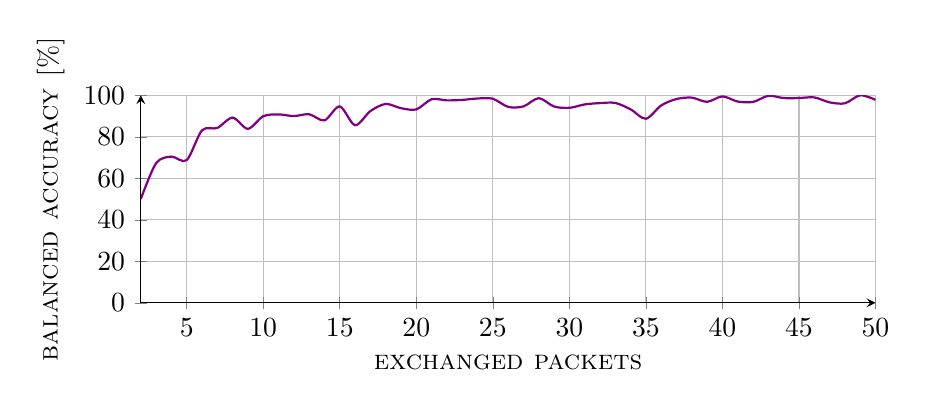
\begin{tikzpicture}
		\begin{axis}[xlabel=\textsc{exchanged packets}, ylabel=\textsc{balanced accuracy [$\%$]}, axis lines=left, grid=major, width=0.9\linewidth, height=12em, ymax=100, ymin=0]
			\addplot +[mark=none, Purple, thick, smooth] table {
				2.0 50.0
				3.0 67.26746714914927
				4.0 70.45817428732478
				5.0 68.73162614056683
				6.0 83.08888313034466
				7.0 84.26442448391528
				8.0 89.24861214775946
				9.0 83.82593657355807
				10.0 89.89600858089419
				11.0 90.78236822880874
				12.0 89.97357623150371
				13.0 90.85193838698513
				14.0 87.9074432369022
				15.0 94.62952849107293
				16.0 85.5770122941313
				17.0 92.36951979858695
				18.0 95.81450967649515
				19.0 93.76805198920685
				20.0 93.1837535326491
				21.0 98.07317331637789
				22.0 97.53939011627072
				23.0 97.76220070337716
				24.0 98.4453914141414
				25.0 98.32424197749276
				26.0 94.41112776944861
				27.0 94.63731479530931
				28.0 98.60709041325782
				29.0 94.5864931338389
				30.0 93.94883557287649
				31.0 95.58719433719433
				32.0 96.22624989055248
				33.0 96.298087758534
				34.0 93.2220397737639
				35.0 88.68480725623583
				36.0 95.10877994444678
				37.0 98.19483348895113
				38.0 98.86363636363636
				39.0 96.8501064153238
				40.0 99.45504087193461
				41.0 96.96830851470027
				42.0 96.79175864606329
				43.0 99.74358974358975
				44.0 98.65994686669791
				45.0 98.65900383141762
				46.0 98.97619047619047
				47.0 96.58899020601149
				48.0 96.13235926085088
				49.0 100.0
				50.0 97.79968315437422
			};
		\end{axis}
	\end{tikzpicture}
	\caption{Balanced accuracy vs. exchange packets plot for the category classifier based on neural network on the KTS.}
	\label{fig:packets_category_neural_network}
\end{figure}
\begin{table}[H]
	\centering
	\begin{subtable}{.45\linewidth}
		\centering
	\begin{tabular}{ll}
		\toprule
		\textsc{inferred class} & \textsc{samples}\\
		\midrule
		browser & 3366\\
		crawler & 358\\
		dos & 2810\\
		\bottomrule
	\end{tabular}
	\caption{Classification of \textsc{firefox-68.0}.}
	\end{subtable}
	\begin{subtable}{.45\linewidth}
		\centering
	\begin{tabular}{ll}
		\toprule
		\textsc{inferred class} & \textsc{samples}\\
		\midrule
		browser & 2012\\
		crawler & 835\\
		dos & 818\\
		\bottomrule
	\end{tabular}
	\caption{Classification of \textsc{grabsite-2.1.16}.}
	\end{subtable}
	\begin{subtable}{.45\linewidth}
		\centering
	\begin{tabular}{ll}
		\toprule
		\textsc{inferred class} & \textsc{samples}\\
		\midrule
		browser & 6086\\
		crawler & 738\\
		dos & 2126\\
		\bottomrule
	\end{tabular}
	\caption{Classification of \textsc{opera-62.0.3331.66}.}
	\end{subtable}
	\begin{subtable}{.45\linewidth}
		\centering
	\begin{tabular}{ll}
		\toprule
		\textsc{inferred class} & \textsc{samples}\\
		\midrule
		browser & 5201\\
		crawler & 3447\\
		dos & 2347\\
		\bottomrule
	\end{tabular}
	\caption{Classification of \textsc{slowhttptest-1.6}.}
	\end{subtable}
	\caption{Classification of unknown tools for the category classifier based on neural network.}
	\label{tab:unknown_category_neural_network}
\end{table}
